\chapter{Solutions to BGD TSTST Problems}\label{sols:tstst}


\section{Solutions to \nameref{tstst:combi}}

\subsection*{Solution to \autoref{combi:1}}
\paragraph{First Solution (Mehrab, unedited)}
Let us assume that there is no circle with a radius of 1  unit which has more than 9  points from S  in it. Now let us take the leftmost point of S  in the plane and take it as a centre and draw a circle of radius 1 . Now at most 8 other points can be inside the circle. That means there are at least 10  other points outside the circle. Now again take the left most of the points outside the circle we have just drawn. And we now draw another circle with a radius 1  with that point as the centre. The new circle can have at most 8 points that are not present in our first circle. So now we have a point in S  that are not in any of the 2 circles we have drawn. But If we take that rogue point and the centre of the 2 circles then 2 points of those 3 must have a distance less than 1  meaning the rogue point should be inside any one of the 2 circles. A contradiction. 


\paragraph{Second Solution (Nayer,unedited)}
Let $G$ be a graph with $19$ vertices and by an edge between any two vertices we mean that they are less than. 1 unit apart.

Let $G'$ be the complement of the graph $G$. Then that means in $G'$, an edge between any two points means that they are At least $1$ unit apart. Now ATQ there cannot be any clique of size $3$  in $G'$ (otherwise that would imply that we would get a triangle in
$G$ with no edge which is impossible)

So, By Turan's theorem, $G'$ can have at most $\frac{1}{2}\times \frac{19^2}{2} \sim 90 $ edges. That means $G$ has $\binom{19}{2}−90 =81$  edges.

By handshake lemma, sum of degree of vertices $\ge 81\times 2=162$. 

By pigeonhole principle there must exist a vertex in G with at least degree $\frac{162}{19} \sim 9$

WLOG suppose that vertex is $V$ Now draw a circle with radius $1$ with centre $V$. So at least $9$ other points are enclosed by that circle.

\subsection*{Solution to \autoref{combi:2}}

\subsection*{Solution to \autoref{combi:3}}


\subsection*{Solution to \autoref{combi:4}}

\subsection*{Solution to \autoref{combi:5}}
%(Solution from Olympiad Combinatorics)
Suppose we have an empty board, and we want to create an arrangement of $k$ checkers satisfying (a) and (b). Call a square good if it contains a checker or shares a side with a square containing a checker. By (a), every square must eventually be good. Let us place the checkers on the board as follows: place one checker on the board to start, and then in each step place one checker adjacent to one that has already been placed. Since any arrangement of checkers that satisfies the problem must be connected by (b), we can form any arrangement of checkers in this manner. 

In the first step at most 5 squares become good (the square we placed the checker on and its neighbors). In each subsequent step, at most 3 squares that are not already good become good: the square we just put a checker on and the square next to it are already good, leaving 3 neighbors that could become good. Thus, at the end of placing k checkers, at most $5+3(k-2) = 3k+2$ squares  are good. But we know all $n^2$ squares are good at the end, so $n \le 3k+2$, proving the result.








\section{Solutions to \nameref{tstst:nt}}


\subsection*{Solution to \autoref{nt:1}}

\subsection*{Solution to \autoref{nt:2}}


\subsection*{Solution to \autoref{nt:3}}







\section{Solutions to \nameref{tstst:geo}}

\subsection*{Solution to \autoref{geo:1}}

\begin{figure}[ht]
\centering
	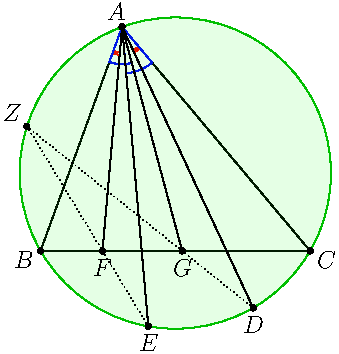
\includegraphics{geo-1.pdf}
\end{figure}
First of all, there are tons of similar triangles. You should find them. We left the angle chasing for the readers as these are good  exercises. 

Note that, $\triangle CAG$ and $\triangle EAB$ is directly similar. Hence, 
\[ AE \cdot AG = AB \cdot AC \ldots (1) \]

Then show that, $\triangle BAF$ and $\triangle DAC$ are similar. So, 
\[ AD \cdot AF = AB \cdot AC \ldots (2)  \]
From (1) and (2) we get, 
\[  AE \cdot AG = AD \cdot AF \ldots (3) \]
So, $\triangle AEF \sim \triangle ADG$. 
Hence, $\angle AEF = \angle ADG.$

Then, we get $\triangle EAD \sim \triangle FAG.$ 

After some angle chase (left as an exercise) we  get the result that, $\angle EZD = \angle EAD$, and therefore $Z$ lies on the  circle.

\subsection*{Solution to \autoref{geo:2}}

\begin{figure}[ht]
\centering
	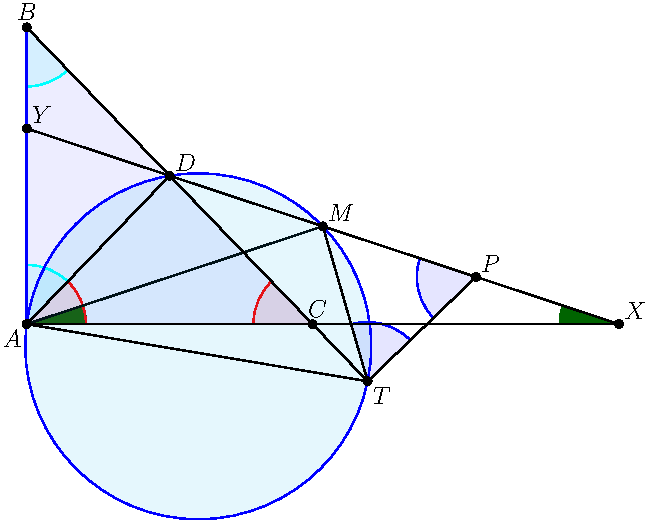
\includegraphics{geo-2.pdf}
\end{figure}

$BD=CD=AD$ ,
$MX=MA=MY$ and
$MD=MP=MT$ 
as $\triangle PTD$ is right angled.
So, $\angle MDT=\angle MTD$
$= \angle BDX = 180 -\angle BXD - \angle DBX =180 - (\angle BAY +\angle AYX ) - \angle DAB $
$=180 -(90+\angle MAC)- \angle DAB =90 -(\angle MAC + \angle DAB)$
 $\boxed{= \angle DAM =\angle DTM} $
$\implies ADMT $ is cyclic. hence $\angle MDT =\angle MTD $
$\implies \angle MAT =\angle MAD$ which implies $AM$ bisects the desired angle. 

\subsection*{Solution to \autoref{geo:3}}
\begin{figure}[ht]
\centering
	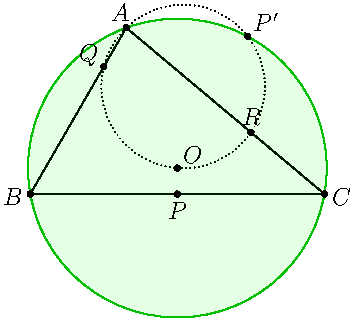
\includegraphics{geo-3.pdf}
\end{figure}

Let $P'$ be the reflection of $P$ over $QR$.
then, $QP=QP'=QB$ and 
$RP=RP'=RC$
$\angle RP'Q=\angle QPR=180 -\angle B -\angle C=\angle A$
So, $PQP'A$ is cyclic.
So,$\angle P'QA=\angle P'RA$, and $P'Q=BQ$, $P'R=CR$.
So, $\triangle P'QB,  \triangle P'RC$ are similar.
Hence $$\angle P'BA= \angle P'BQ=\angle P'CR=\angle P'CR=\angle P'CA$$.
Which results in $BPCA$ is cyclic.
Now $$\angle P'OQ=\frac{1}{2} P'OB=\angle P'CB=\angle P'AB=\angle P'AQ=\angle P'RQ$$
Hence $P'QOR$ is cyclic. we proved $P'QRA$ cyclic before. 
So $AQOR$ is cyclic.


\subsection*{Solution to \autoref{geo:4}}
\begin{figure}[htb]
\centering
	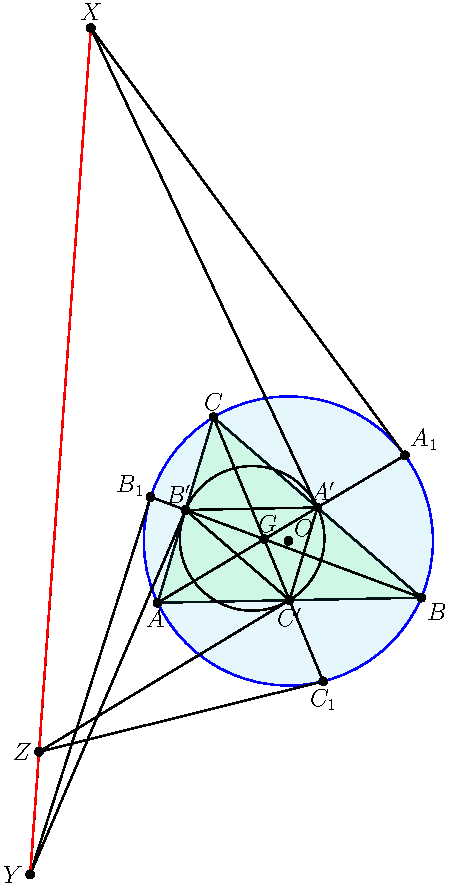
\includegraphics[scale=.8]{geo-4.pdf}
\end{figure}
Solution thanks to Luis Gonz\'{a}lez.

Centroid $G = AA' \cap BB' \cap CC'$ of $\triangle ABC$ is the insimilicenter between its circumcircle $(O)$ and $9$-point circle $(N)$. $A, A'$ are homologous under such homothety implies tangent $\nu$ of $(N)$ at $A'$ is parallel to the tangent $\tau$ of $(O)$ at $A$. Which implies $\nu$ is antiparallel to $BC$ $\implies  A'X \equiv \nu$. The lines $\tau, XA_1$ and $AA_1$ bound an isosceles triangle, therefore $\triangle XA'A_1$ is isosceles with apex $X$ implies $X$ has equal power with respect to $(O)$, $(N)$. Which implies $X$ lies on the radical axis of $(O), (N)$, i.e. the orthic axis of $\triangle ABC$. Analogously, $Y, Z$ lie on the orthic axis of $\triangle ABC$.


